
% ---------------------------------------------
\chapter{Dust Modeling Images}
\label{chap: Appendix_DustModels}





\section{Porous Spherical Grain Model}

Here, I have included an additional plot showing \Pweff versus maximum grain size as in Figure \ref{fig:Pweff_vs_grainsize} (left), but for a porous spherical grain. 


% ----------------------------------------------------------------
\begin{figure}[htbp]
  \centering
  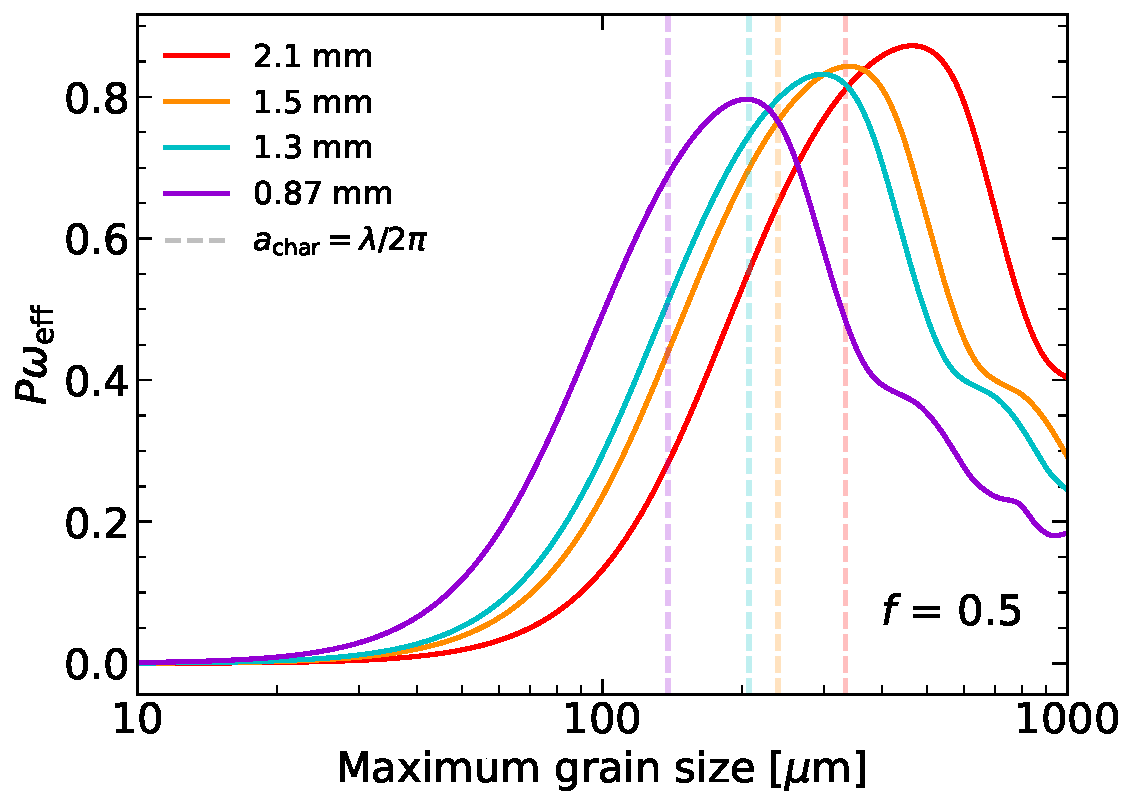
\includegraphics[width=0.5\textwidth]{WRITEUP_AND_IMAGES/IMAGES/WRITEUP/DustModels/Pw_eff_vs_grainsize_porous_smooth.pdf}
  \caption{Same as Figure \ref{fig:Pweff_vs_grainsize} (left, spherical) but for a porous grain. } 
  \label{fig: Pweff_vs_amax_porous}
\end{figure}
% ----------------------------------------------------------------



\section{Additional Spherical Grain Models}



Additional plots with results comparing \Pwmodel curves and \POLFsi are presented below. Figure \ref{fig: Spherical_BEST}, presented in Chapter \ref{sec: chapter5_spherical_dust_model_results}, shows the best-fit results when \bfive is excluded for filling factors of $f = 1.0, 0.5, 0.3$ and $0.1$. Figure \ref{fig: appendix_nob5_extra_porosities} presents the same fitting case for the remaining porosities. Figure \ref{fig: appendix_all_band} shows the results when all wavelengths are included in the fit, while Figure \ref{fig: appendix_just_47} shows the results when only \bfour and \bseven are included. Figures \ref{fig: appendix_all_band} and \ref{fig: appendix_just_47} include results for all filling factors. 



\begin{figure}[htbp]
  \centering
  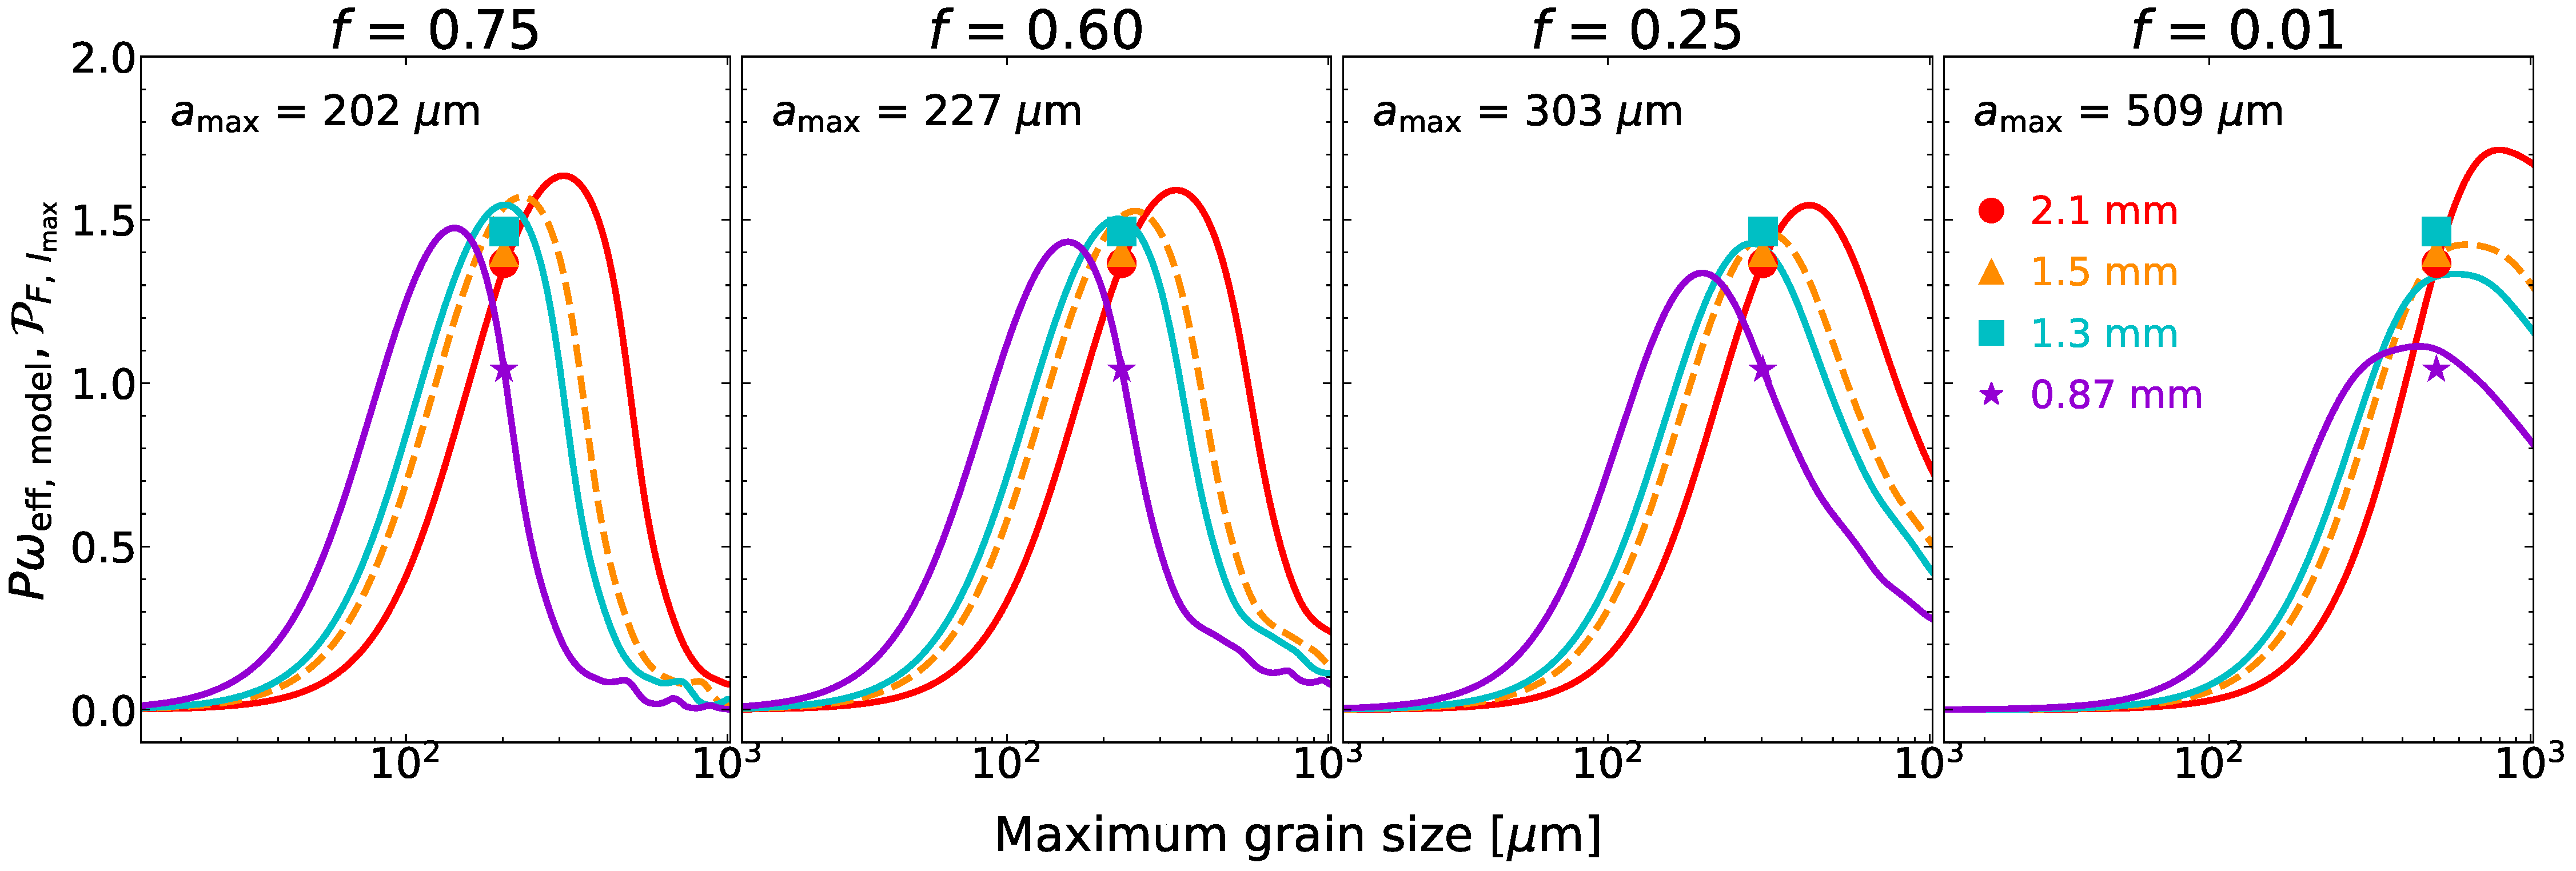
\includegraphics[width=0.99\textwidth]{WRITEUP_AND_IMAGES/IMAGES/WRITEUP/DustModels/DustModelPlot_Without5_ZhangMethod_Extraf}
  \caption{Same as Figure \ref{fig: Spherical_BEST}, but for the remaining porosities.}
  \label{fig: appendix_nob5_extra_porosities}
\end{figure}




\begin{figure}[htbp]
  \centering
  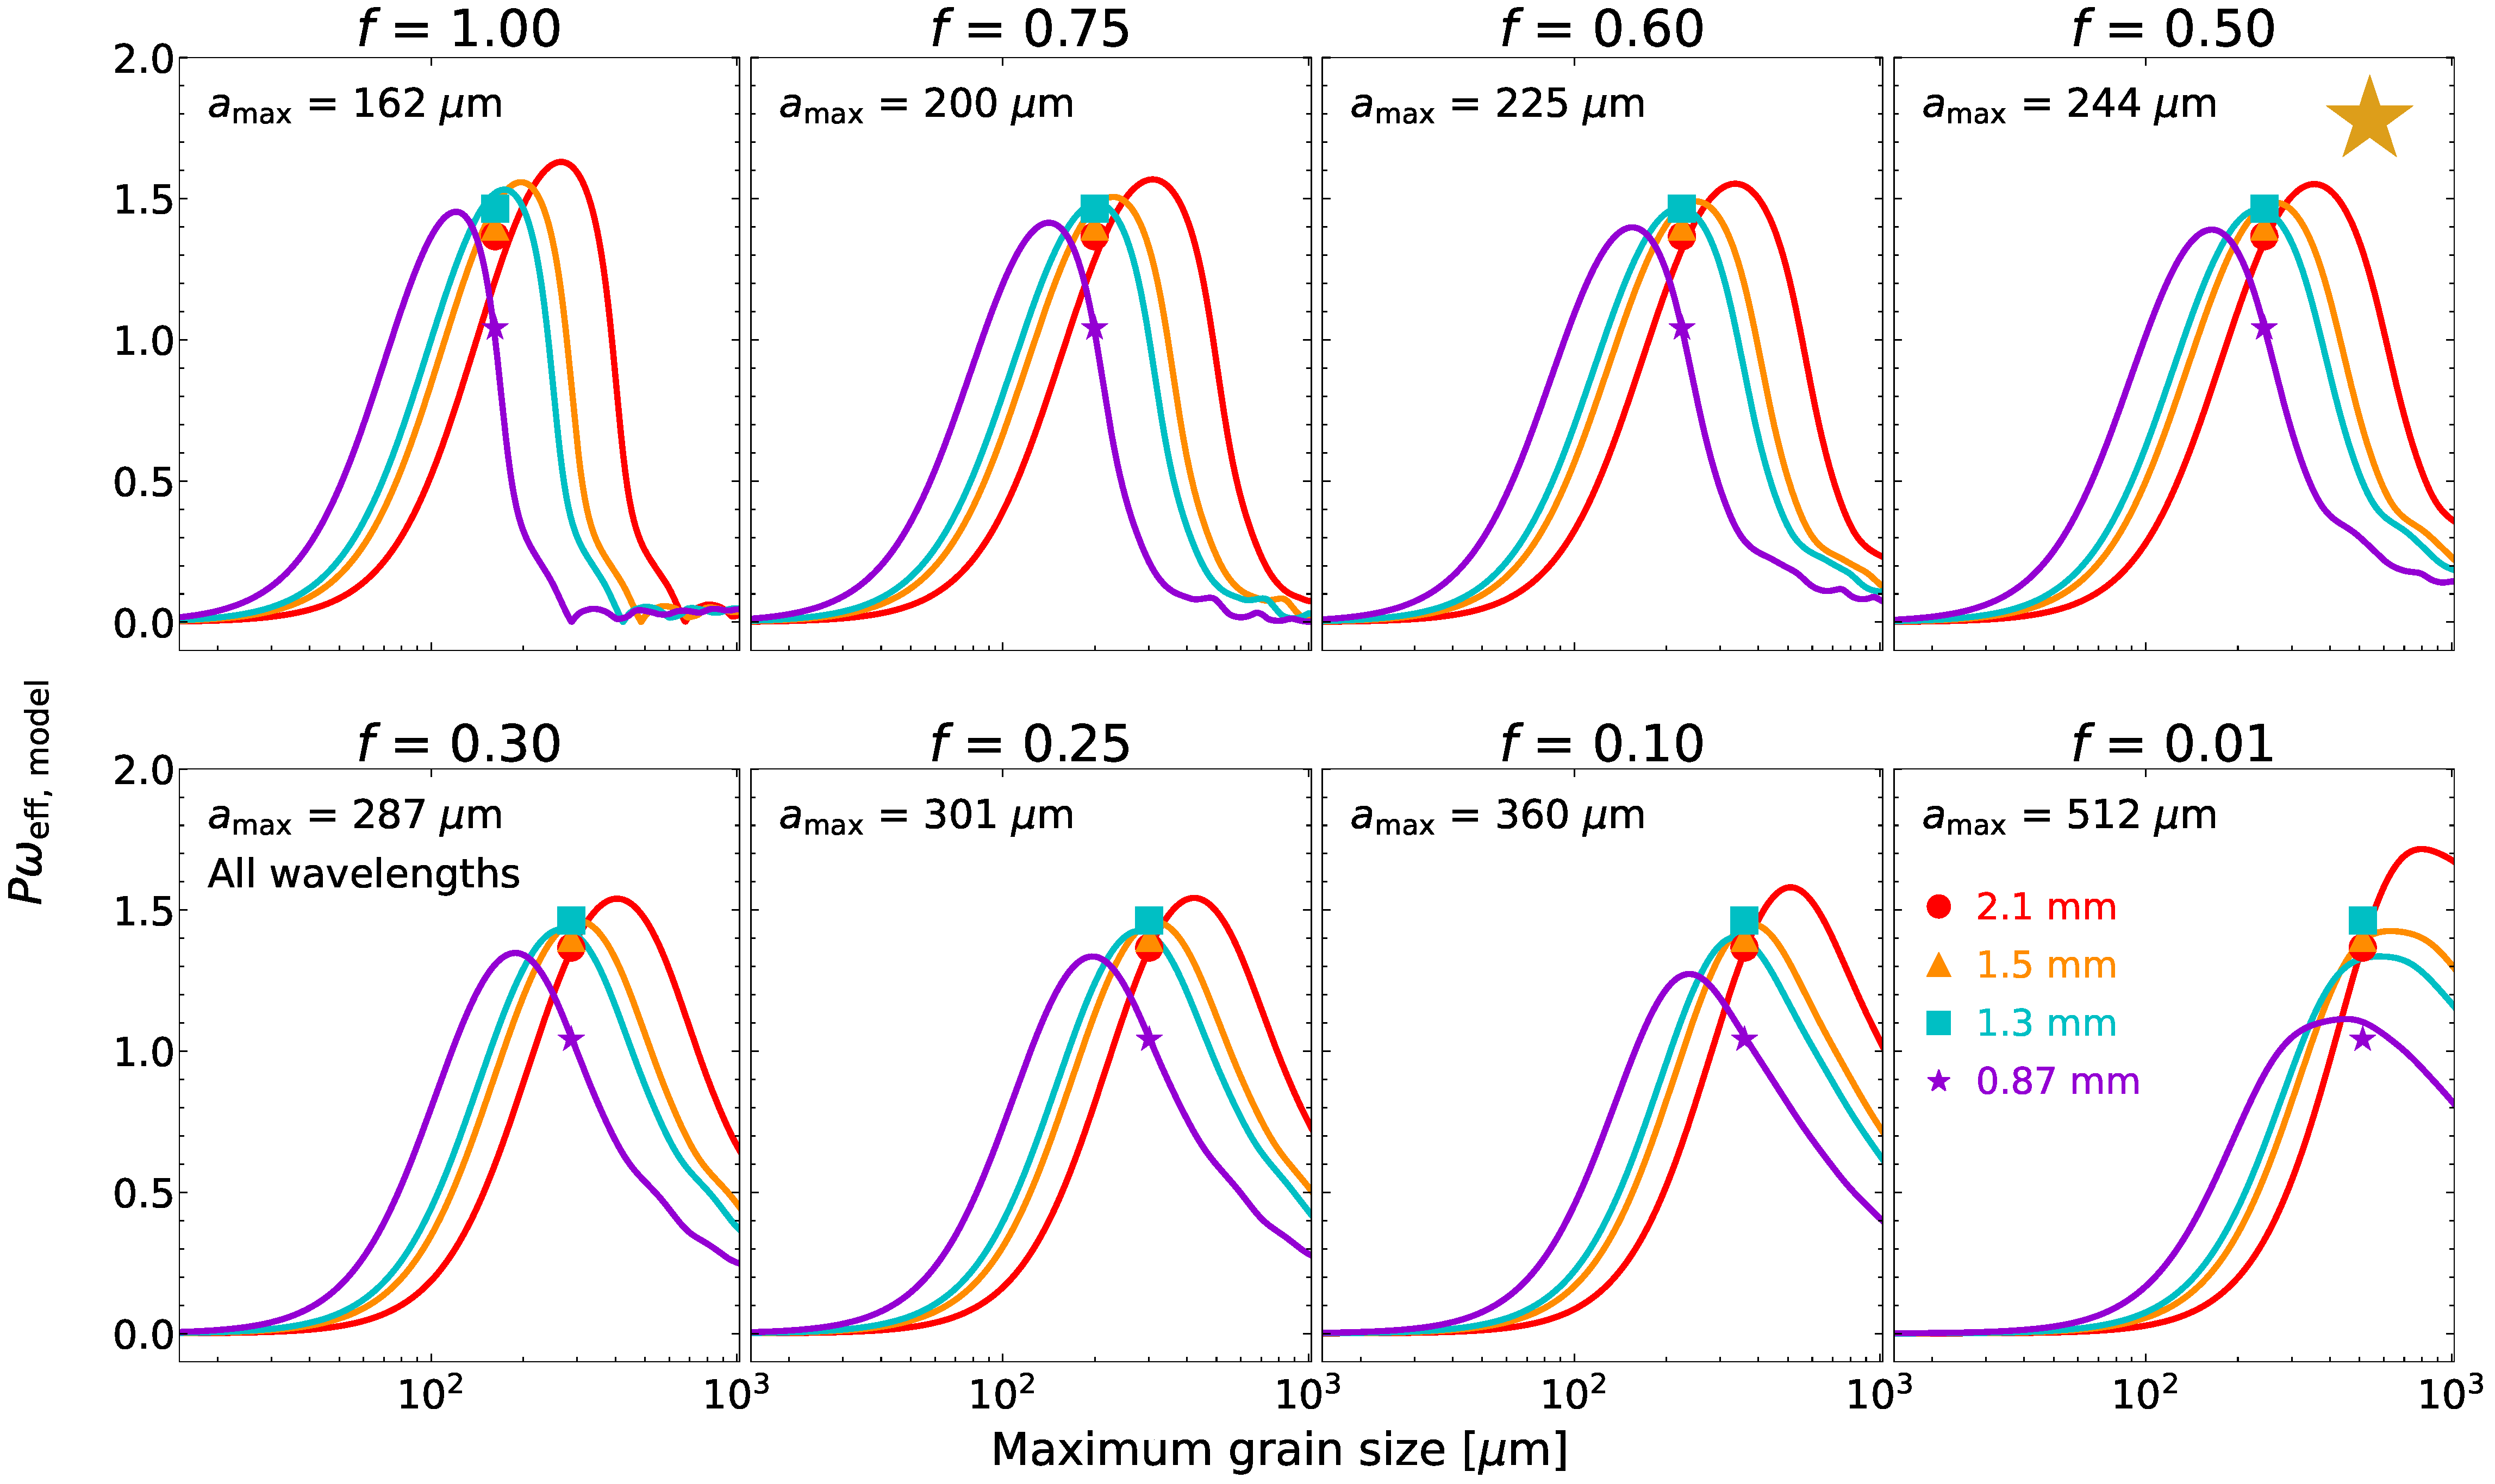
\includegraphics[width=0.99\textwidth]{WRITEUP_AND_IMAGES/IMAGES/WRITEUP/DustModels/DustModelPlot_AllBands_ZhangMethod_ALL.pdf}
  \vspace{0.5cm}
  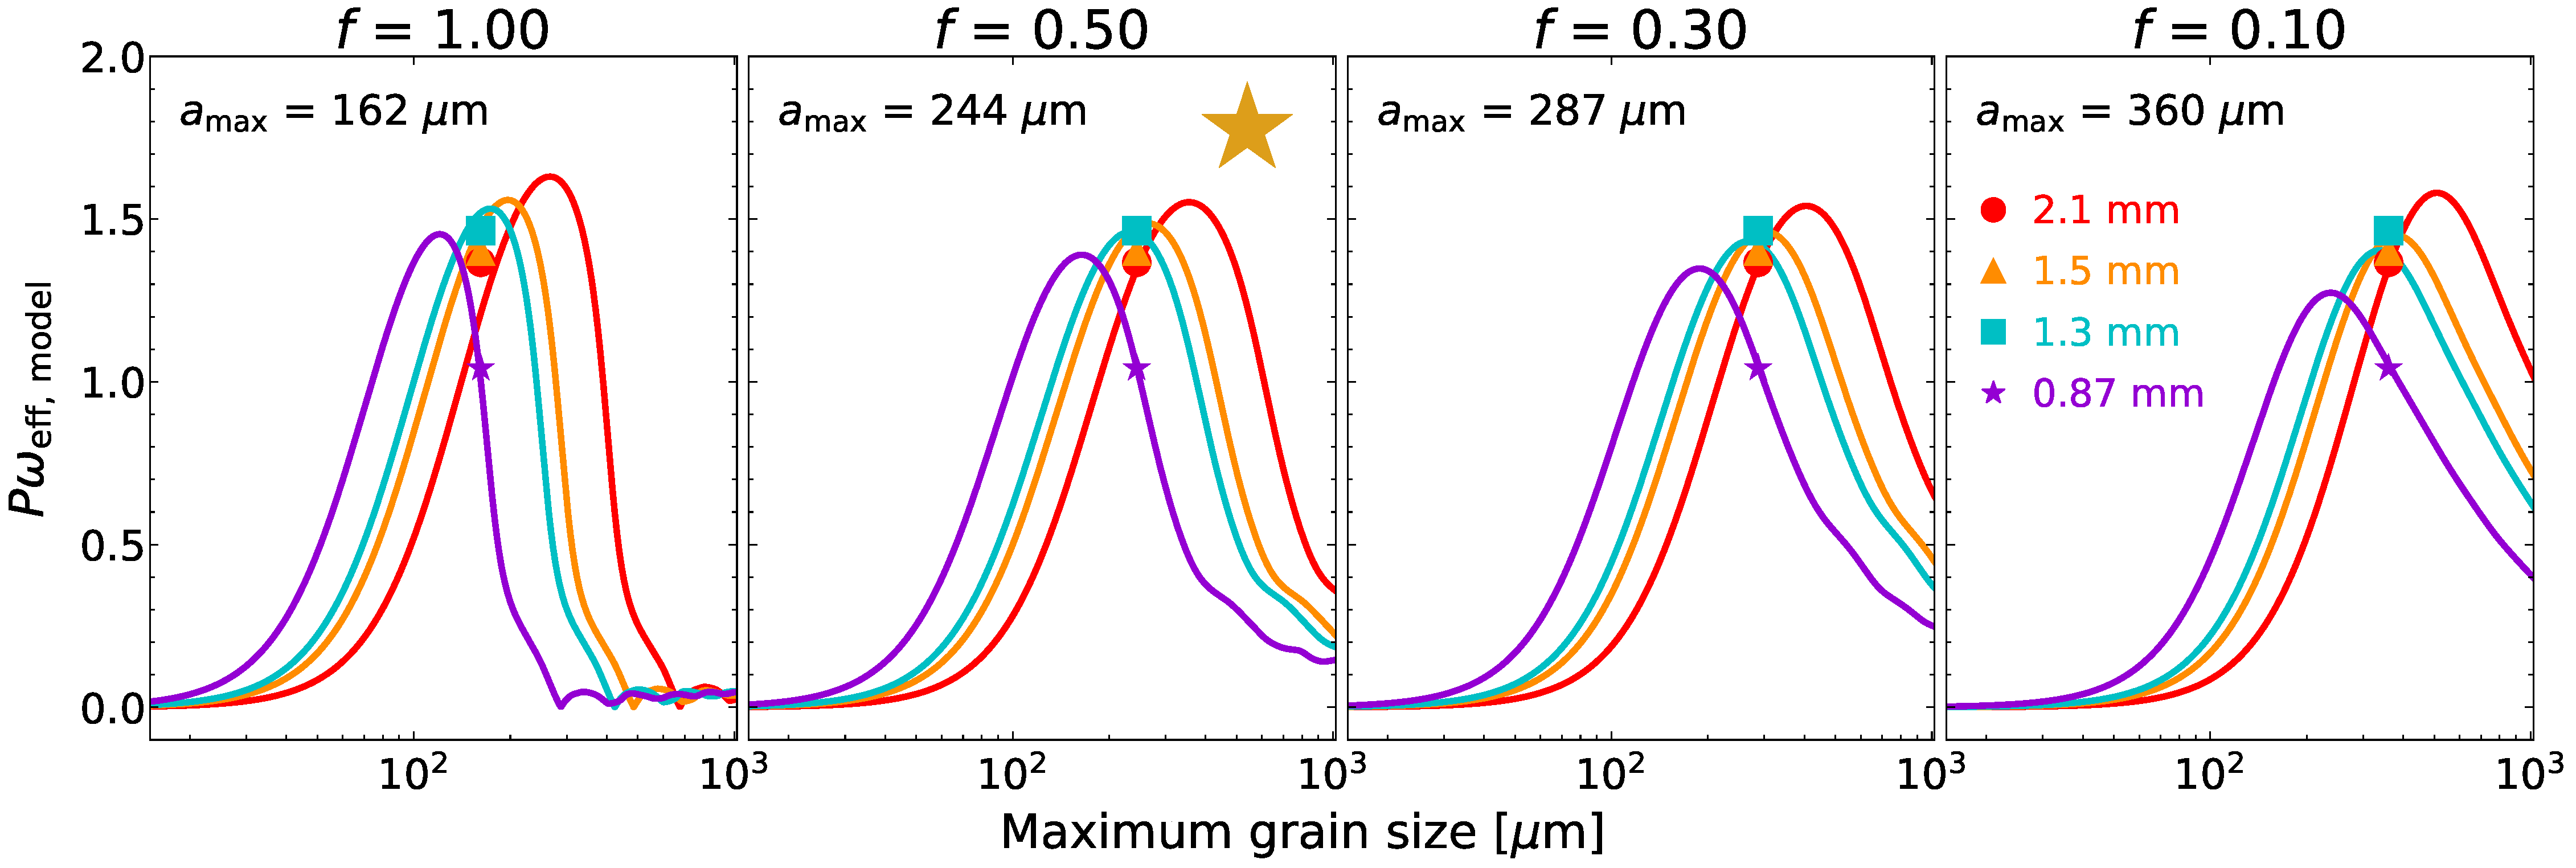
\includegraphics[width=0.99\textwidth]{WRITEUP_AND_IMAGES/IMAGES/WRITEUP/DustModels/DustModelPlot_AllBands_ZhangMethod.pdf}
  \caption{Same as Figure \ref{fig: Spherical_BEST}, but for the all wavelengths fit case and all tested porosities.}
  \label{fig: appendix_all_band}
\end{figure}



% \begin{figure}[htbp]
%   \centering
%   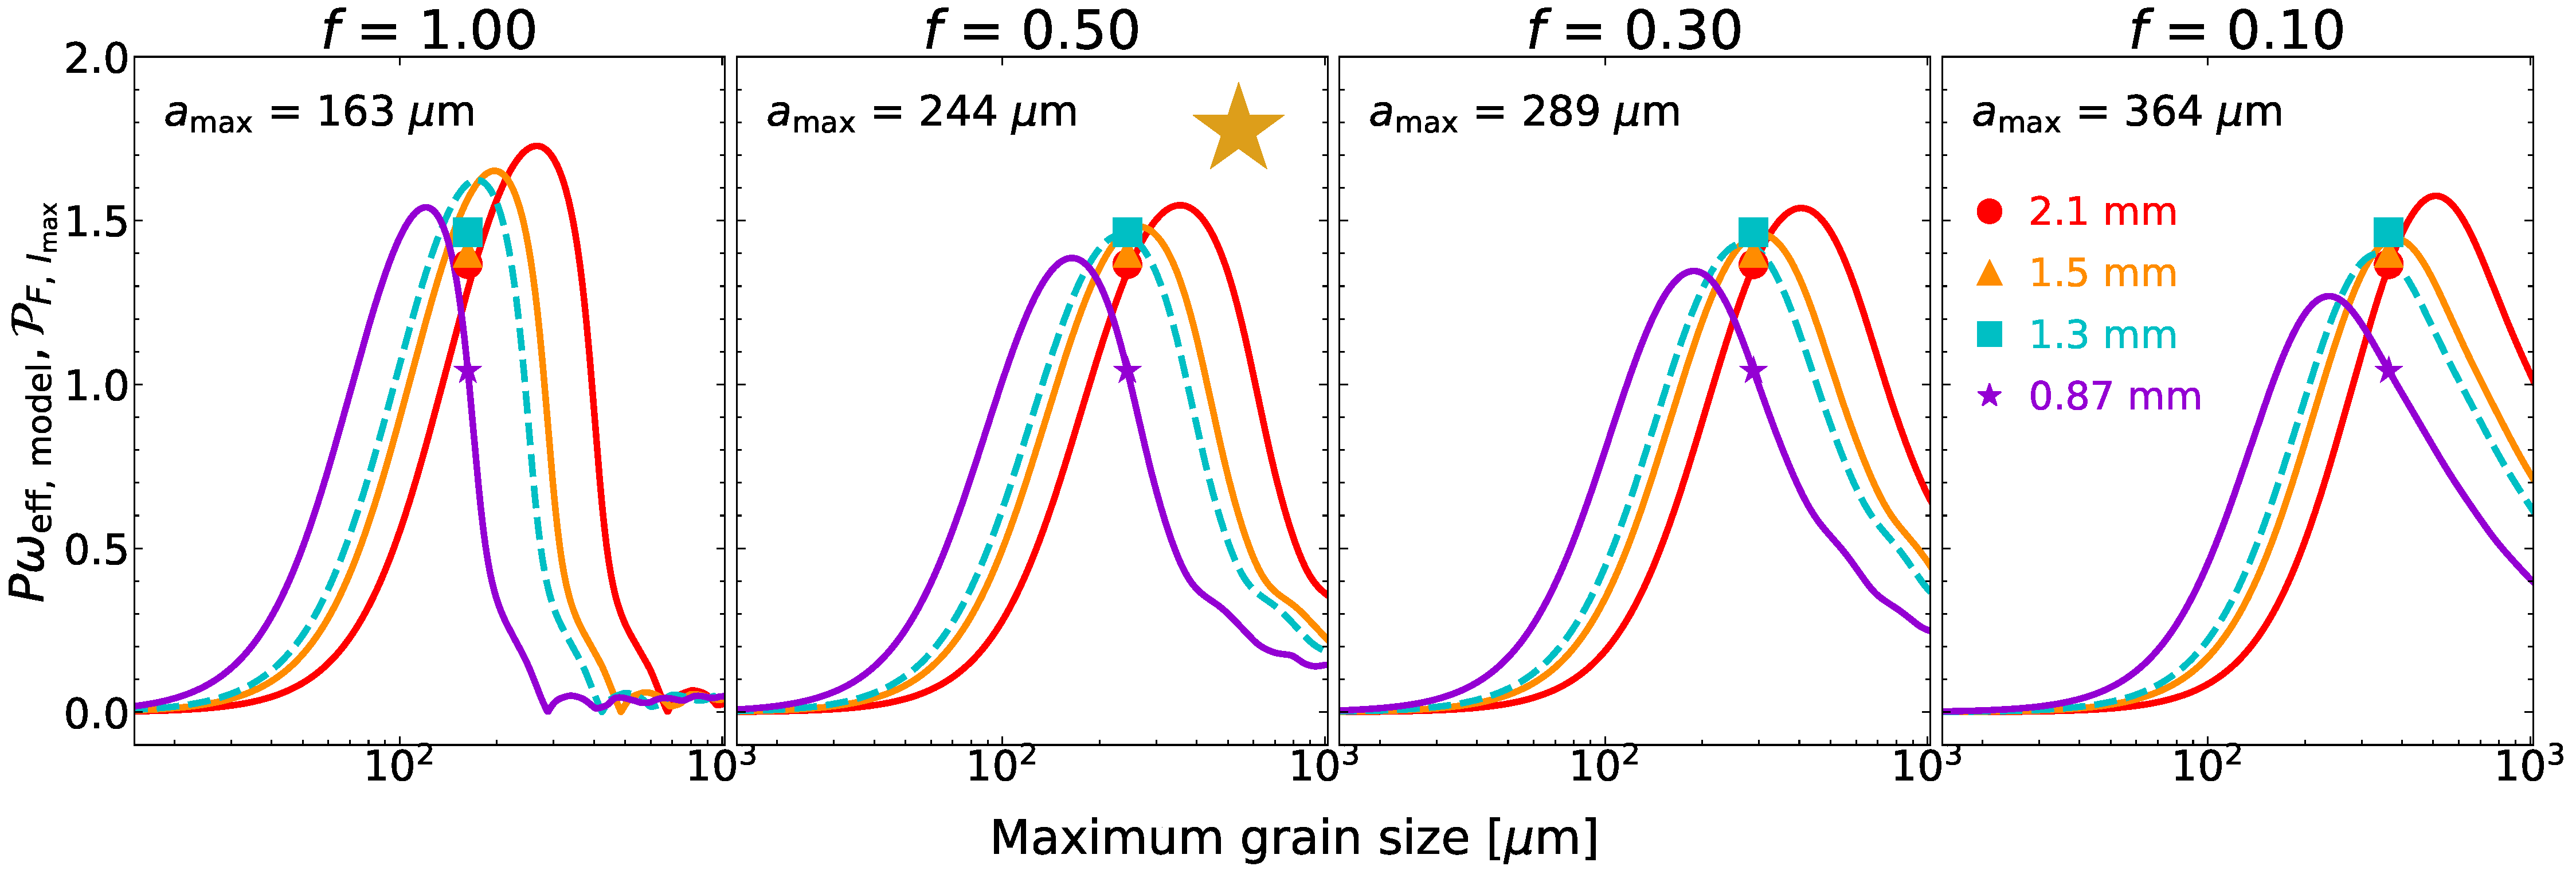
\includegraphics[width=1.1\textwidth]{WRITEUP_AND_IMAGES/IMAGES/WRITEUP/DustModels/DustModelPlot_Without6_ZhangMethod.pdf}
%   \caption{Same as Figure \ref{fig: Spherical_BEST}, but for the no \bsix fit case.}
%   \label{fig: appendix_no6}
% \end{figure}


\begin{figure}[htbp]
  \centering
  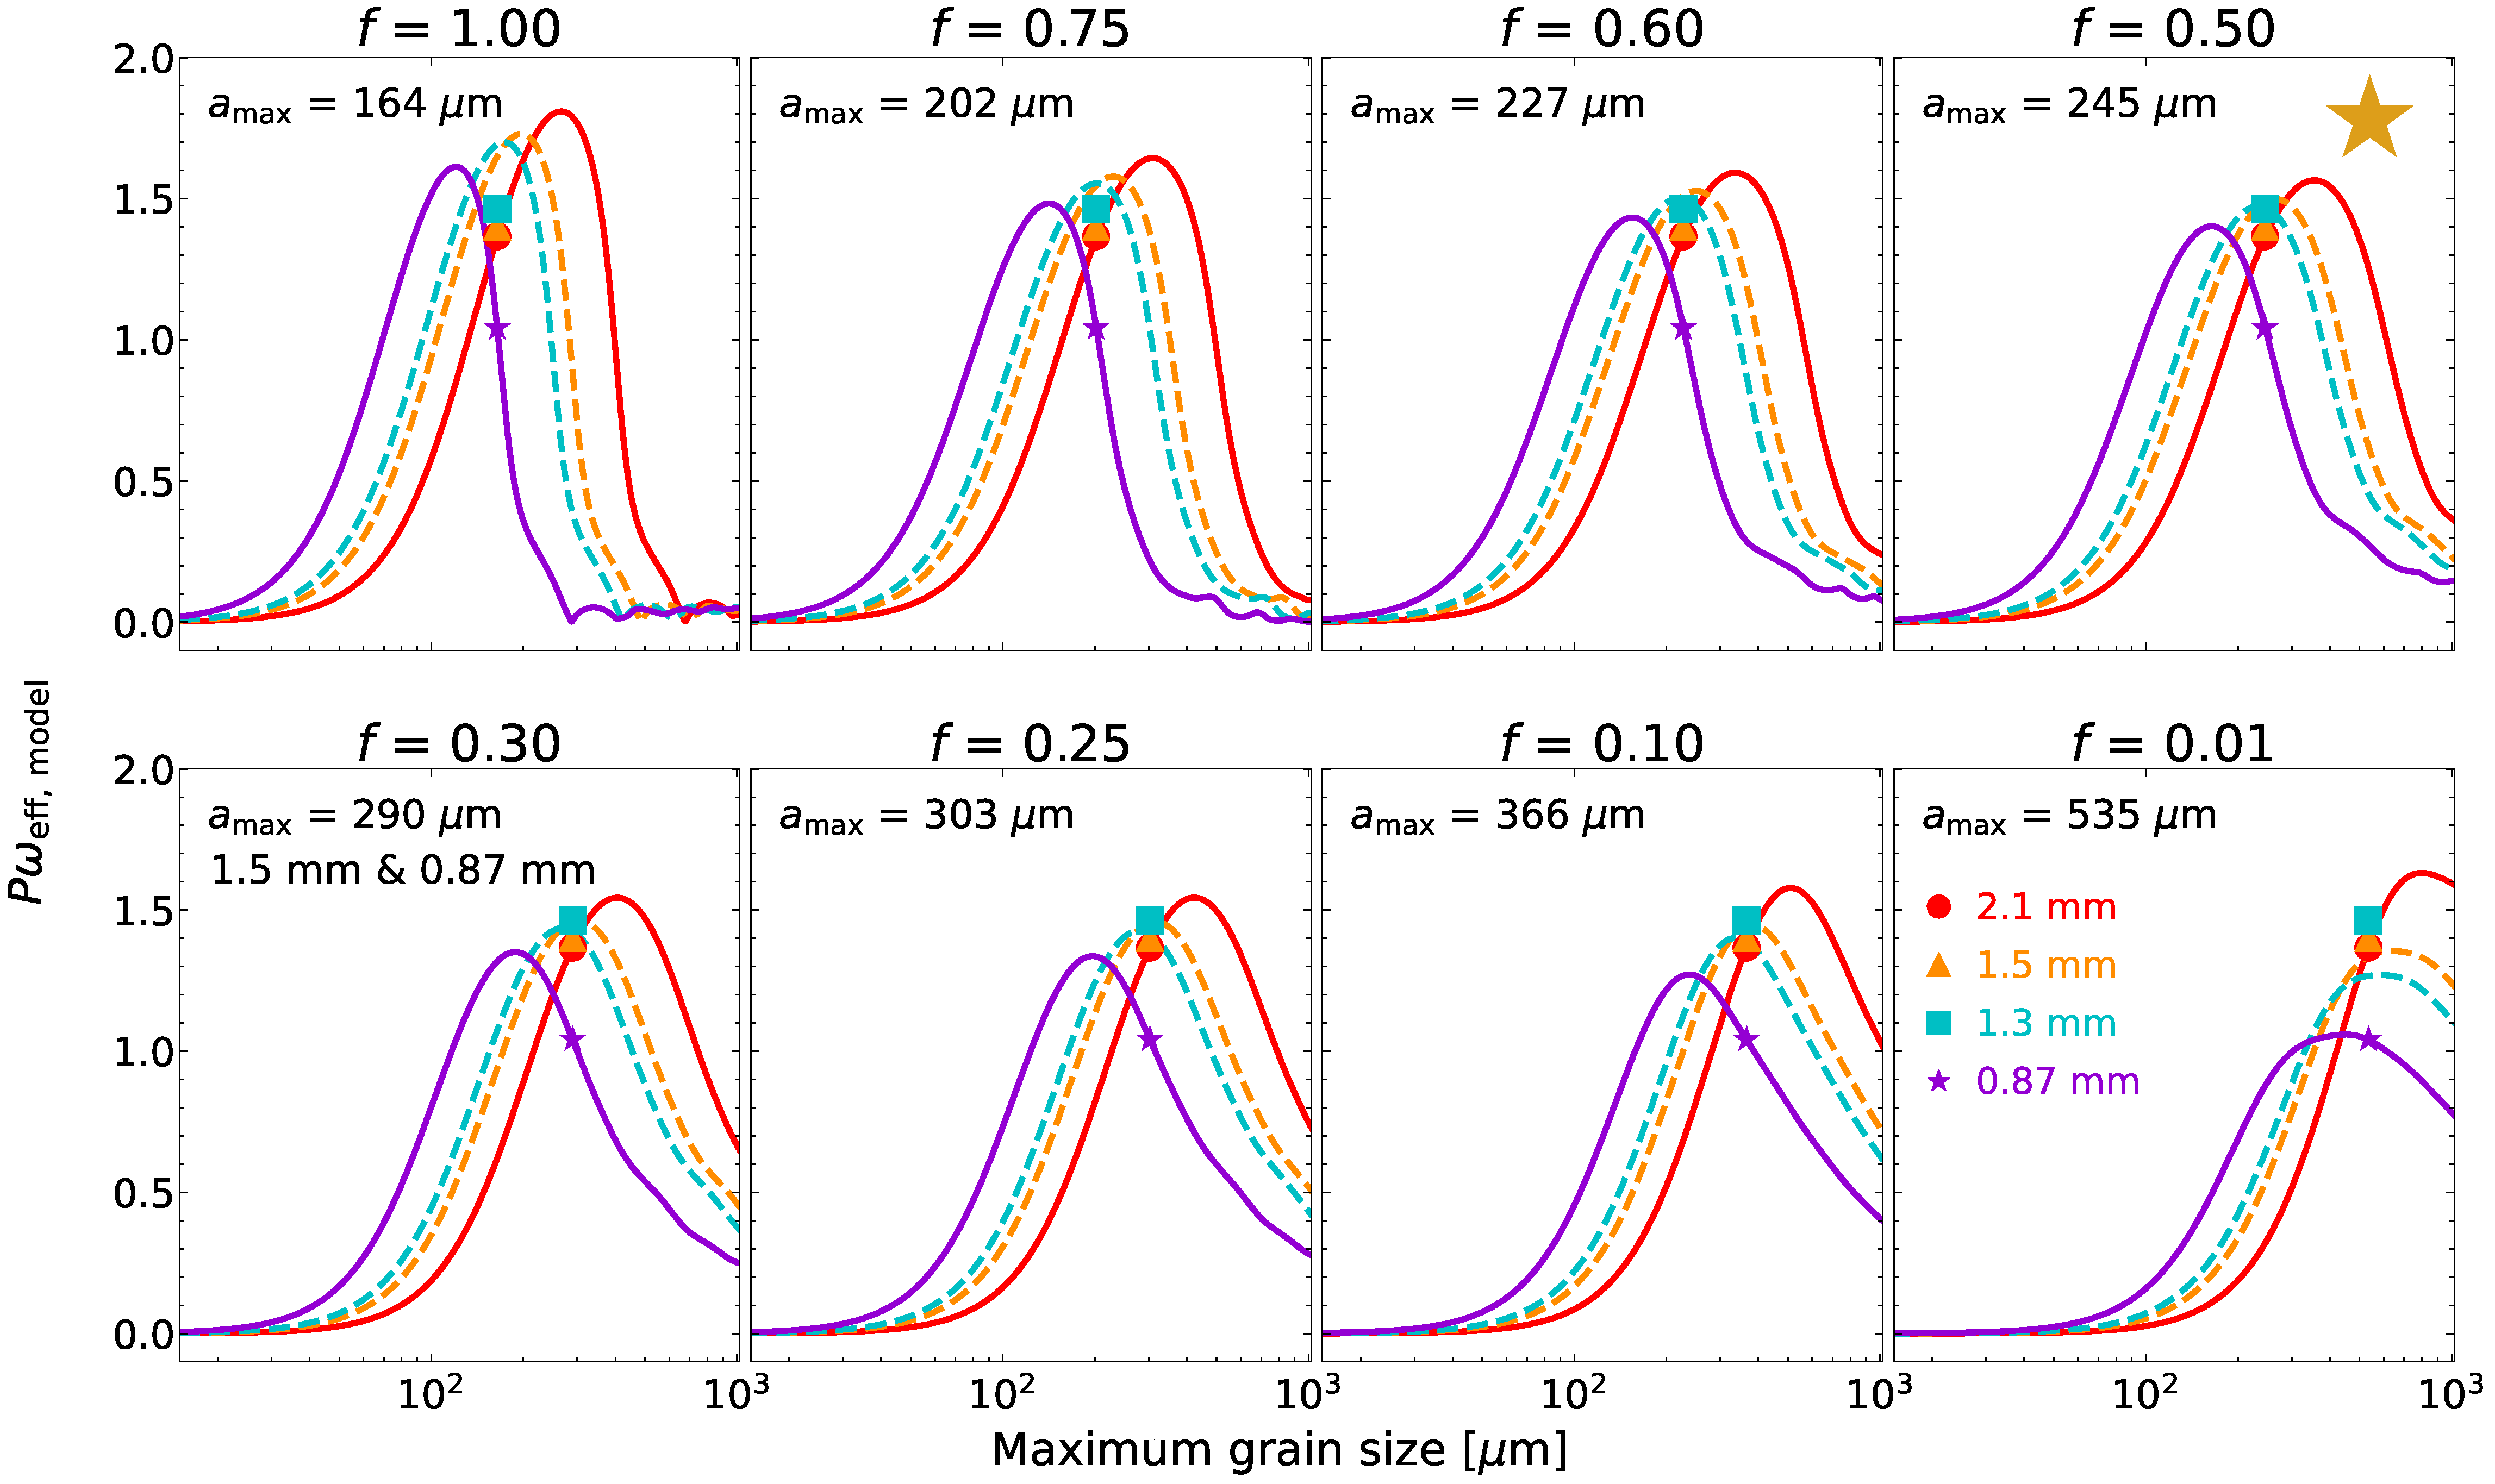
\includegraphics[width=0.99\textwidth]{WRITEUP_AND_IMAGES/IMAGES/WRITEUP/DustModels/DustModelPlot_Just47_ZhangMethod_ALL.pdf}
  \caption{Same as Figure \ref{fig: Spherical_BEST}, but for the just \bfour and \bseven fit case and all porosities. }
  \label{fig: appendix_just_47}
\end{figure}































% ---------------------------------------------


% ---------------------------------------------
% \chapter{\Pw plots}

% % ----------------------------------------------
\begin{figure}[htbp]
  \centering
  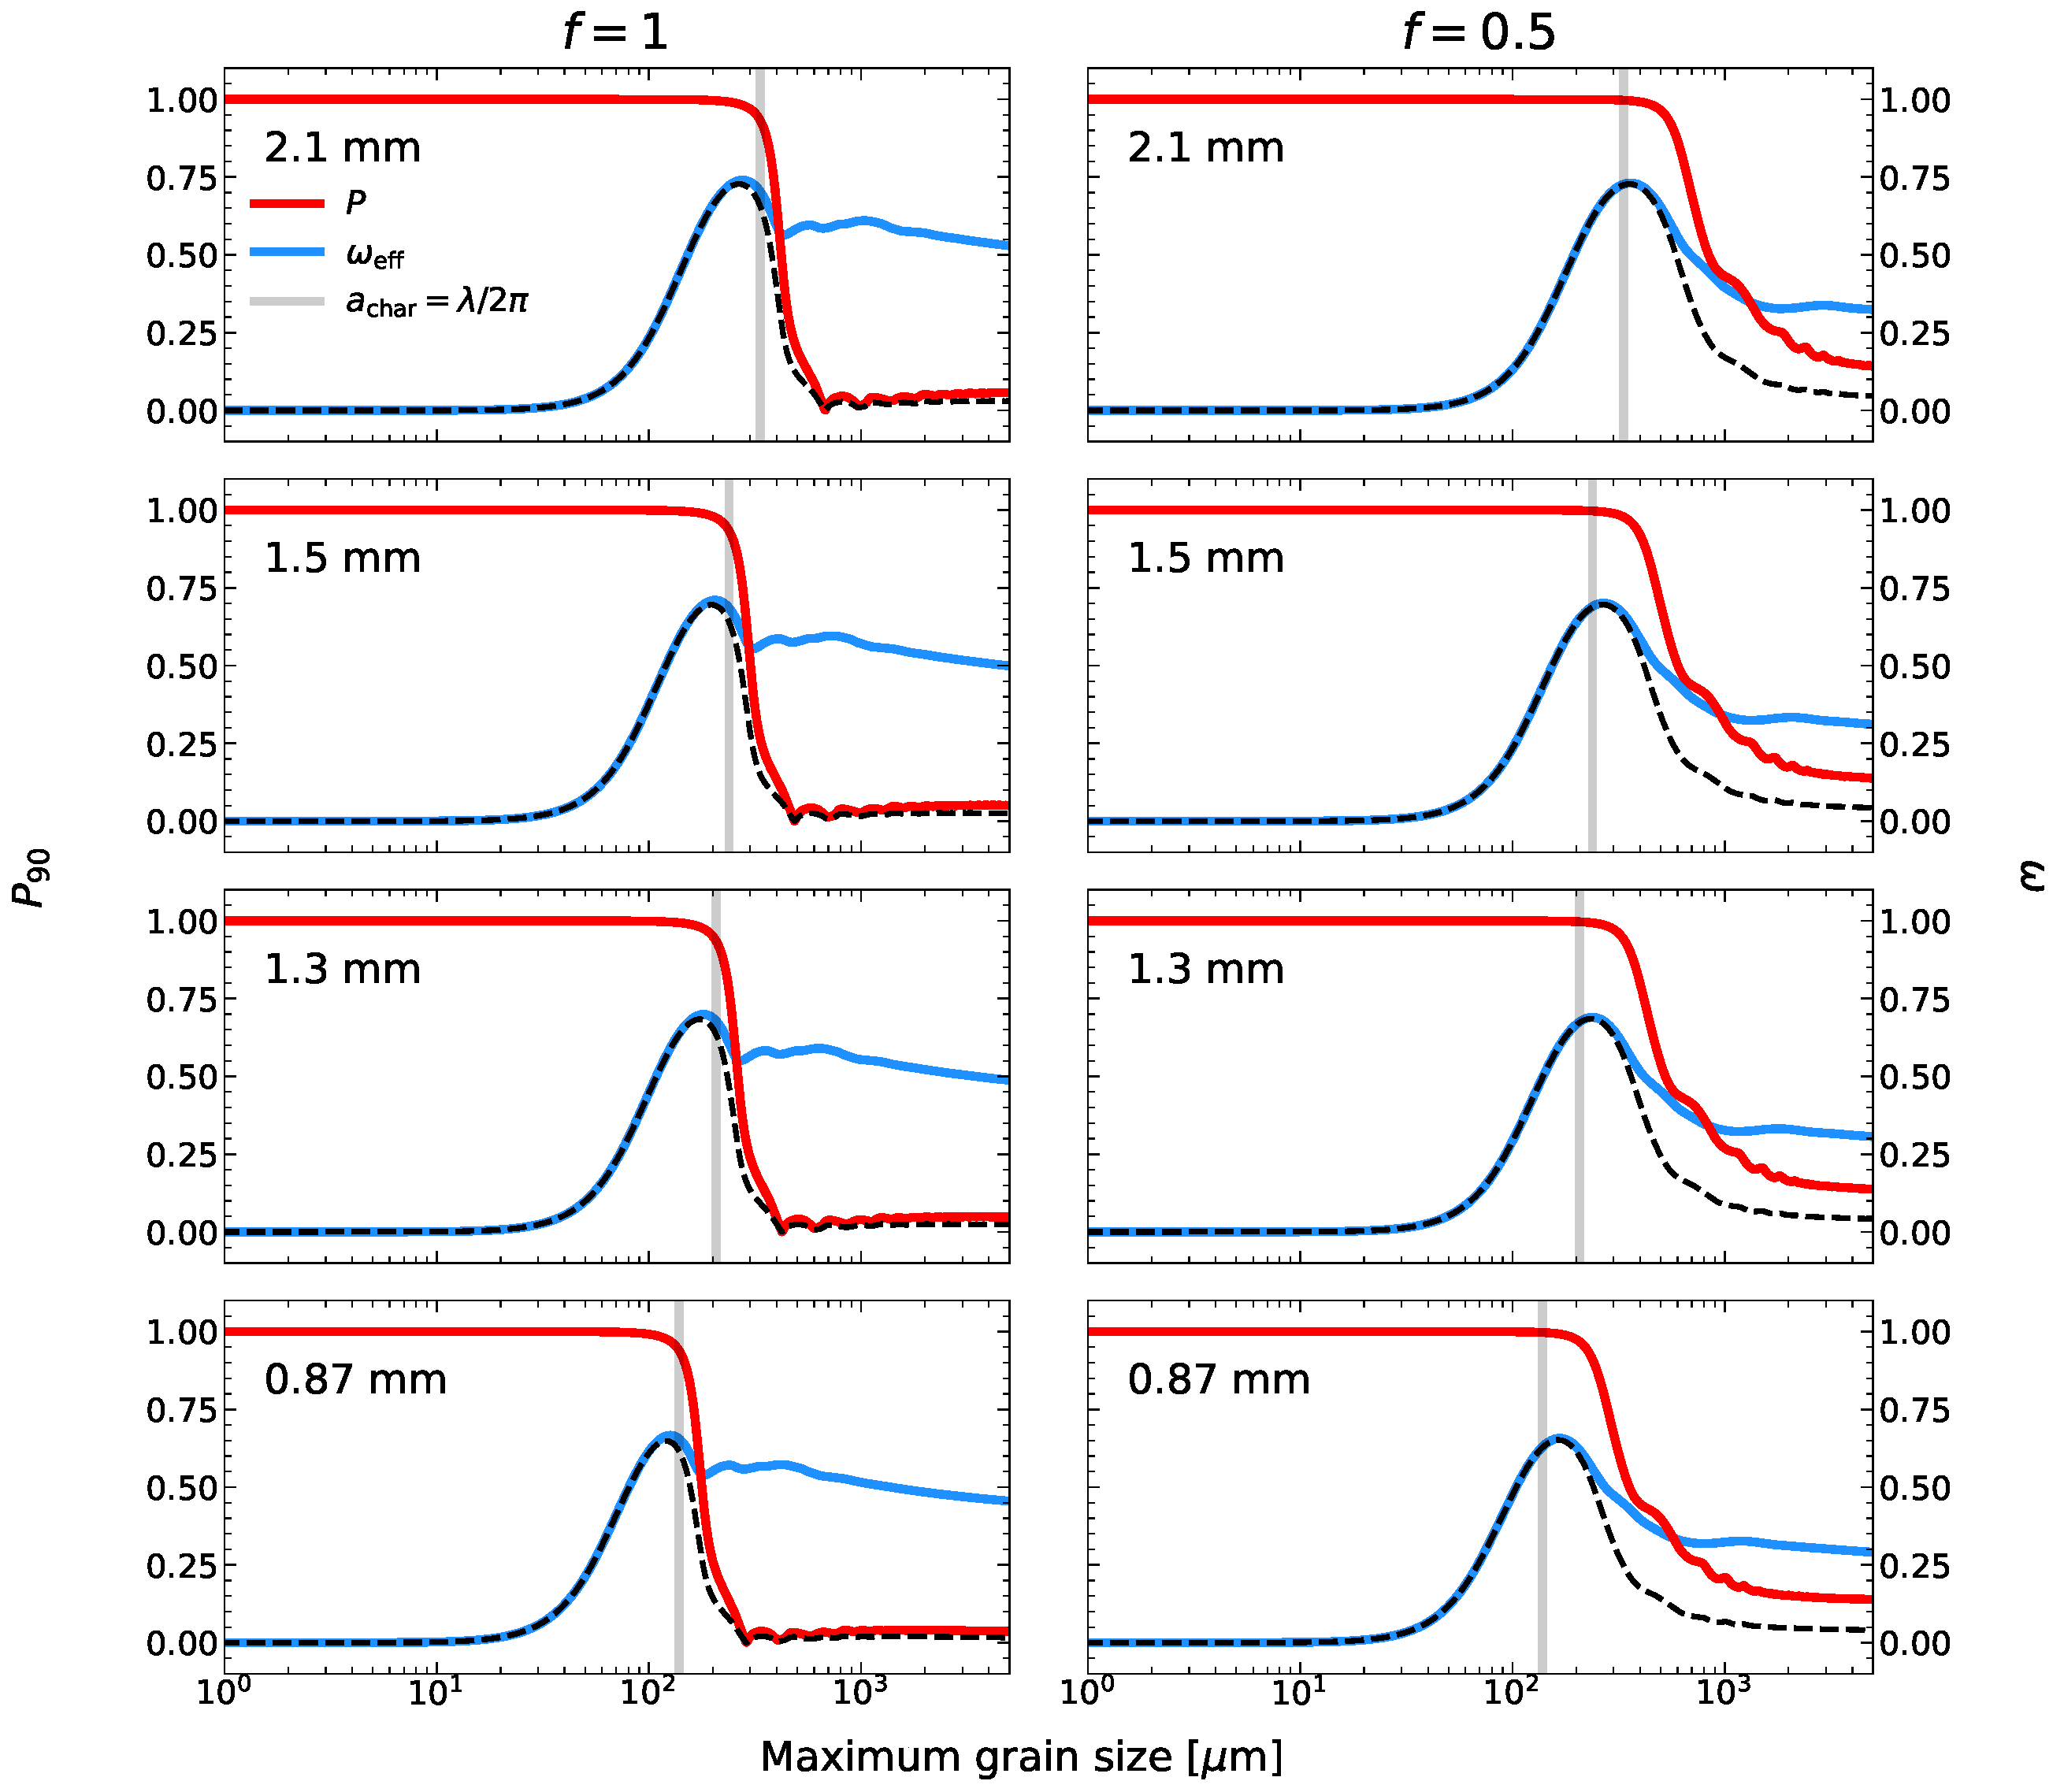
\includegraphics[width=0.99\textwidth]{WRITEUP_AND_IMAGES/IMAGES/WRITEUP/DustModels/P_vs_w_vs_grainsize_grid_smooth_porosities.pdf}
  \caption{Same as Figure \ref{fig: Kataoka2015Figure3Recreation} but for \Pw not \PweffNS.}
  \label{fig: Kataoka2015Figure3Recreation_Pw}
\end{figure}
% ----------------------------------------------


% ------------------------------------------------------
\begin{table}[h!]
\centering
\caption{Same as Table \ref{tab: amax_peak_values} but for \Pw and not \PweffNS. \add{references to plots} \intextref{add}}
%\label{tab:amax_peak_values}
\begin{tabular}{lcccc}
\toprule
\textbf{Grain Size ($\boldsymbol{\mu}$m)} & \textbf{\bfour} & \textbf{\bfive} & \textbf{\bsix} & \textbf{\bseven} \\
\midrule

$a_{\text{char}}$
& 334.23
& 238.73
& 206.90
& 138.46 \\

$a_{\max}$ (spherical)
& 266.02
& 196.46
& 173.46
& 120.70 \\


$a_{\max}$ (irregular)
& 333.19 
& 240.77 
& 213.26 
& 147.62 \\



\bottomrule
\end{tabular}
%\label{tab: amax_peak_values_Pw}
\end{table}
% ------------------------------------------------------



\subsection{\Pw and compact}
% ----------------------------------------------
\begin{figure}[htbp]
  \centering

  \begin{minipage}[t]{0.48\textwidth}
    \centering
    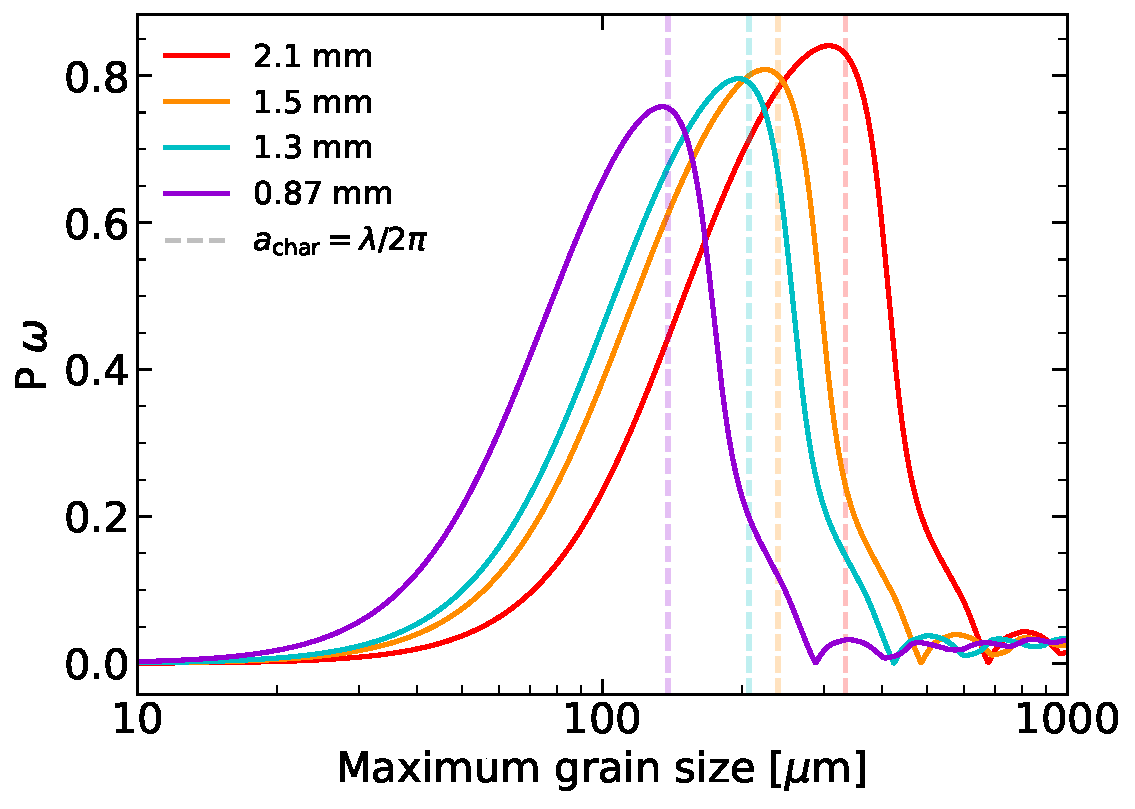
\includegraphics[width=\textwidth]{WRITEUP_AND_IMAGES/IMAGES/WRITEUP/DustModels/Pw_vs_grainsize_smooth.pdf}
  \end{minipage}
  \hfill
  \begin{minipage}[t]{0.48\textwidth}
    \centering
    
\includegraphics[width=\textwidth]{WRITEUP_AND_IMAGES/IMAGES/WRITEUP/DustModels/glitterin/Pw_vs_grainsize.pdf}
  \end{minipage}

  \caption{Same as Figure \ref{fig: Pweff_vs_grainsize} but for \Pw and not \PweffNS.}
  \label{fig: Pw_vs_grainsize_appendix}
\end{figure}
% ----------------------------------------------




% ------------------------------------------------------
\begin{table}[h!]
\centering
\caption{Same as Table \ref{tab: dust_model_fits_irregular} but for fits using $\omega$ and not \weffNS. \refintext{add}}
\begin{tabular}{lccc}
\toprule
\textbf{Fit Case} &  \textbf{Scale Factor (SF)} & $\boldsymbol{\chi_\mathcal{P}^2}$ & \textbf{$\boldsymbol{\amaxEQ}$ ($\boldsymbol{\mu}$m)} \\
\midrule

All wavelengths  & \textbf{1.77} & \textbf{4.58} & \textbf{212} \\
No \bfive               & 1.81 & 6.16 & 214 \\
Just \bfour and \bseven & 1.83 & 8.41 & 215 \\
\bottomrule
\end{tabular}
\label{tab: dust_model_fits_irregular_no_eff}
\end{table}
% ------------------------------------------------------




% ----------------------------------------------------------------
\begin{figure}[htbp]
  \centering
  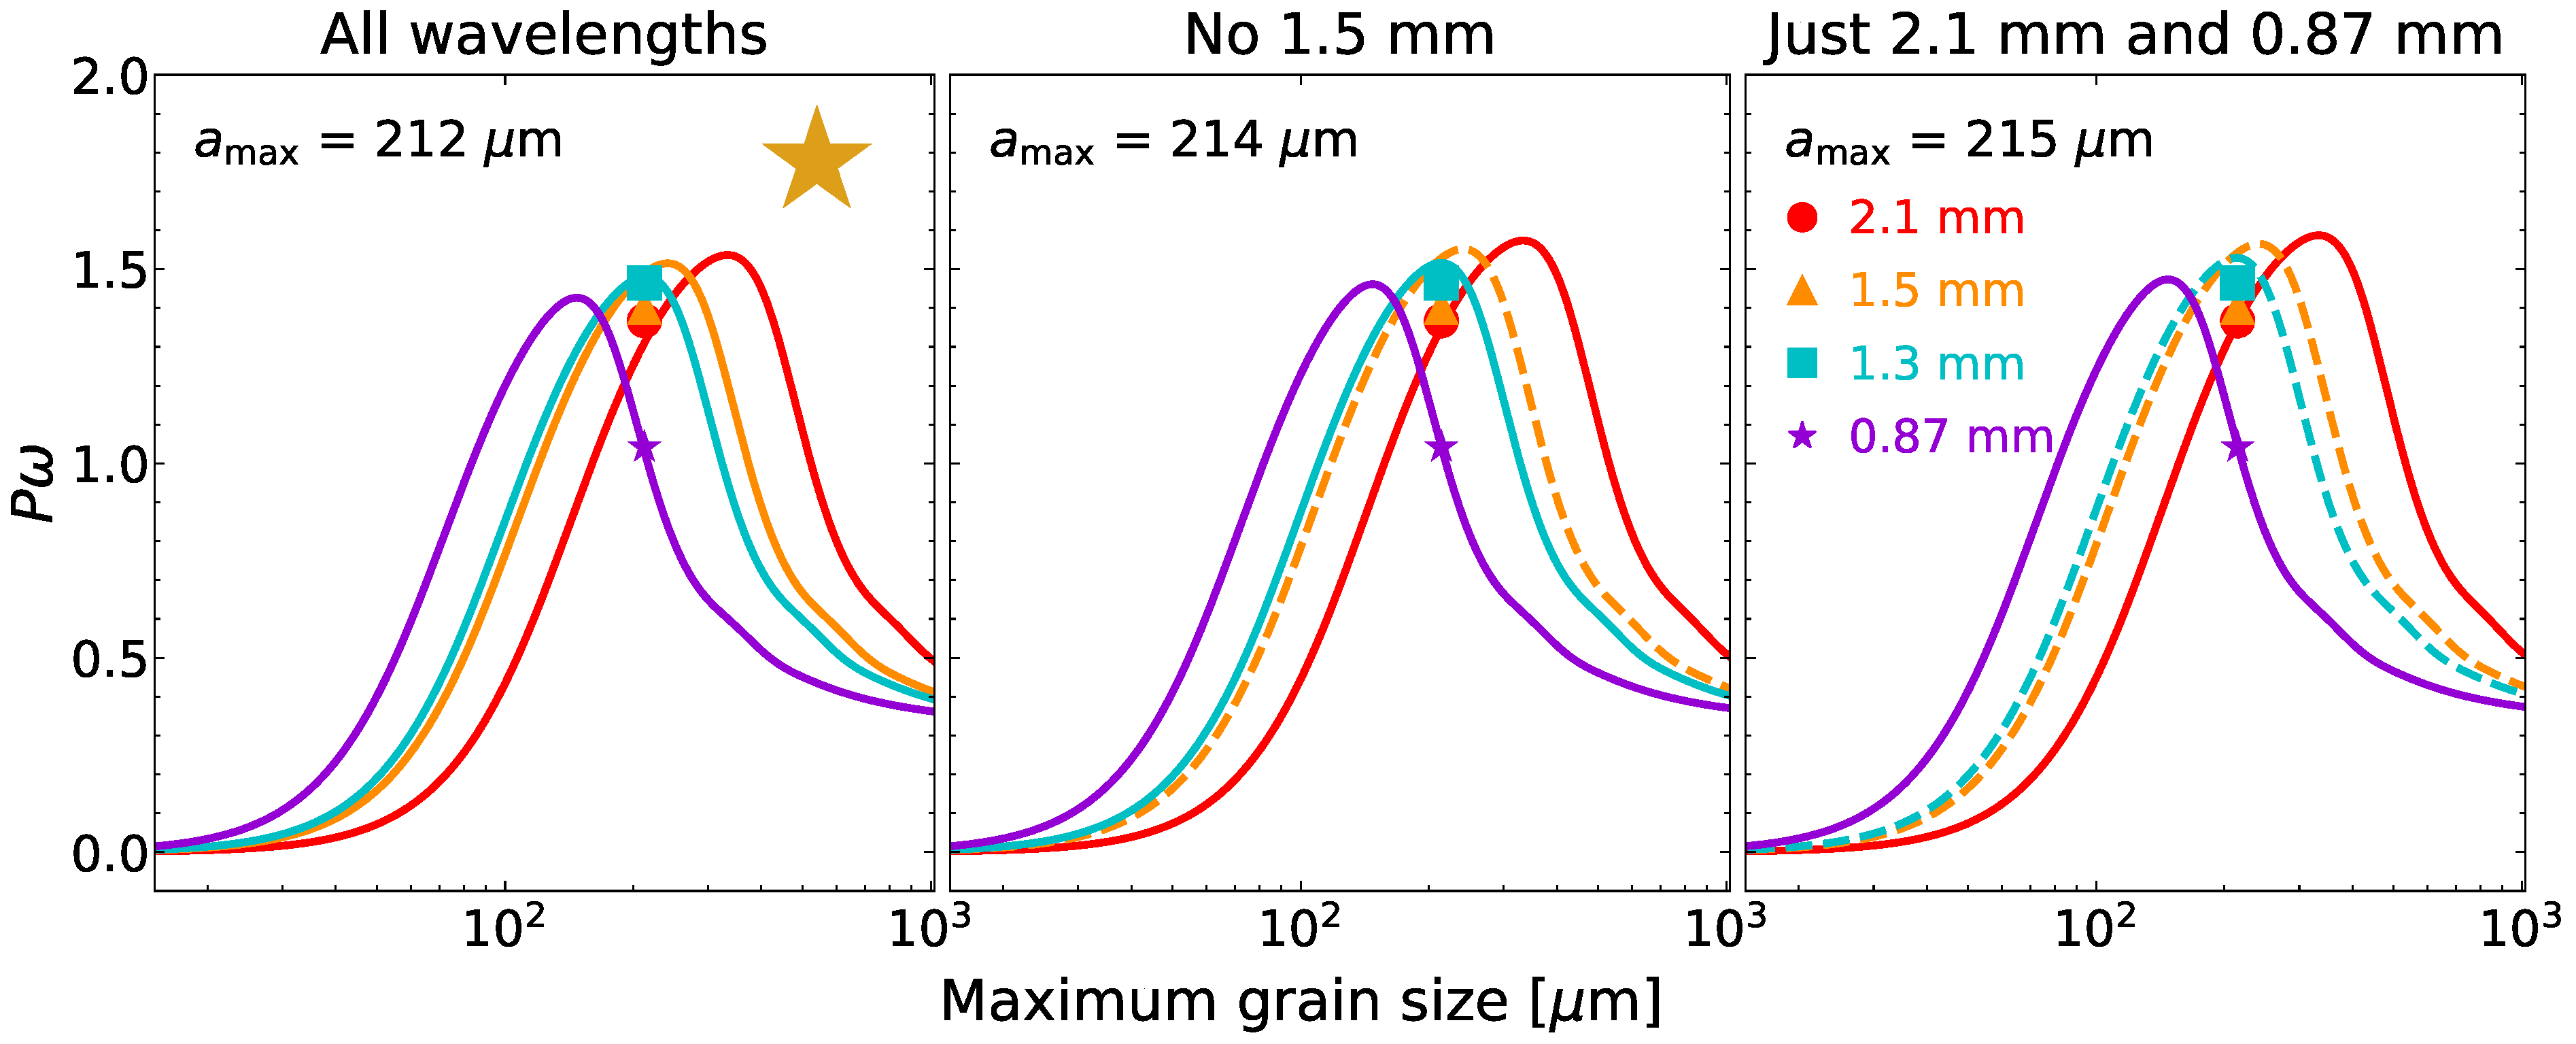
\includegraphics[width=0.99\textwidth]{WRITEUP_AND_IMAGES/IMAGES/WRITEUP/glitterin/DustModelPlot_GlitterinGrid_only3.pdf}
  \caption{Same as Figure \ref{fig: irregular_fits} but for \Pw and not \PweffNS. \code{Change to $P$ not P, wrong panel has star} \refintext{add}} 
  \label{fig: irregular_fits_w}
\end{figure}
% ----------------------------------------------------------------




% ---------------------------------------------


% ---------------------------------------------
% \chapter{Other}

% \subsection{Biased POLF}

% ----------------------------------------------
% ----------------------------------------------
\begin{table}[h!]
\centering
\caption{Same as Table \ref{ref: polf_comparison} but for biased polarization fraction.}
\begin{tabular}{lllll}
\toprule
\textbf{Parameter} & \textbf{\bfour} & \textbf{\bfive} & \textbf{\bsix} & \textbf{\bseven} \\
\midrule

$\mathcal{P}_{\mathrm{F, max\,I}}$
& 1.37
& 1.40
& 1.46
& 1.04 \\

$\mathcal{P}_{\mathrm{F, max\,POLI}}$
& 1.56
& 1.51
& 1.49
& 1.08 \\


$\mathcal{P}_{\mathrm{F, Gaussian}}$
& 1.16
& 1.35
& 1.41
& 0.90 \\

\bottomrule
\end{tabular}
\label{tab: polf_comparison_biased}
\end{table}
% ----------------------------------------------
% ----------------------------------------------

% ---------------------------------------------